\chapter{Design}\label{design}

This chapter gives a high-level overview of the  design of \texttt{Observer-Controller} architecture used in the KIA4SM project. It also describes the design details of  the \texttt{Synchronization} module and the communication architecture between the \texttt{Synchronization} module and \texttt{Controller} module.

\section{Overview}

\begin{figure}[h]
  \centering
  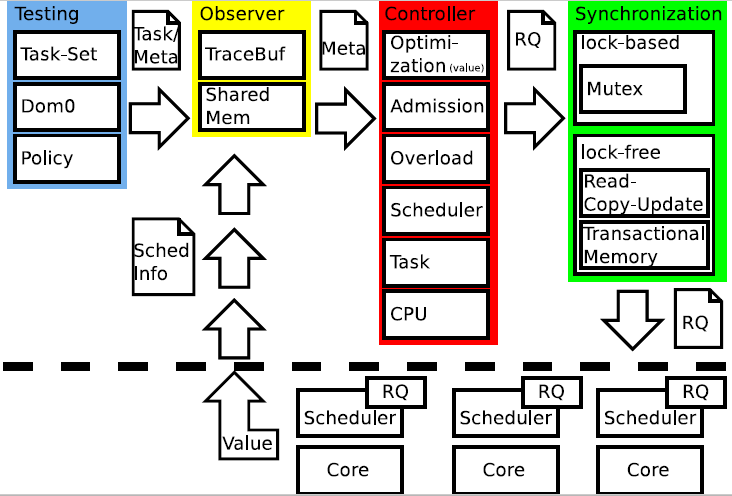
\includegraphics[scale = 0.7]{figures/oc.png}
  \caption{The Observer- Controller architecture}\label{oc}
\end{figure}

The figure \ref{oc} shows the \texttt{Observer-Controller} architecture. Its goal is to have a system that can automatically take the decisions of scheduling tasks/threads by observing the system. There are three main modules involved, namely, \texttt{Observer}, \texttt{Controller} and \texttt{Synchronization}. All these modules are implemented as Genode OS applications (or components).

The \texttt{Observer}'s (also called Monitor/Monitoring agent) job is to collect all the information from the system, analyse it and send it to the \texttt{Controller}. The \texttt{Observer} collects the information by using the \texttt{Trace} facility available in Genode. The data collected from the \texttt{Observer} includes \textit{number of tasks}, \textit{process ID}, \textit{execution time of each task}, \textit{RAM info}, \textit{CPU quota}, etc.

The \texttt{Controller} is responsible for maintaining the system in a safe and optimized state. It analyses the data collected from the \texttt{Observer} and takes a decision for system reconfiguration\cite{kia4sm}. The system reconfiguration involves updating a single thread to the ready queue or generating a new ready queue. It then communicates the system reconfiguration data to the \texttt{Synchronization} module. The \texttt{Controller} also applies load balancing or energy saving techniques to keep the system in an optimized state.

The design of \texttt{Synchronization} component is quite complicated. The initial design consisted of having a high-level component, which can directly access the kernel ready queue and exchange it with the ready queue given by the \texttt{Controller}. This requires synchronized access to the kernel ready queue. However, further research showed that this design required modification due to the following reasons:  

\begin{itemize}
\item Kernel ready queue cannot be directly accessed from a high-level component such as the one proposed, since the kernel protection domain prevents direct access.

\item The \texttt{Controller} cannot create the ready queue that can be directly used by the kernel. This is because the
thread ids represented in Genode OS framework differ from the thread ids in the kernel. Moreover, the ready queue list in the kernel has scheduler context objects in it (explained in \ref{Foundations:rq} and \ref{Foundations:sc}). Hence, a user-level component such as the \texttt{Controller} cannot access scheduler context objects.

\item The list type for ready queue is implemented in a template class called \texttt{Dlist}, which is accessible only from the kernel and needs a re-implementation in the user-level component.

\end{itemize}

\begin{figure}[h]
	\centering
	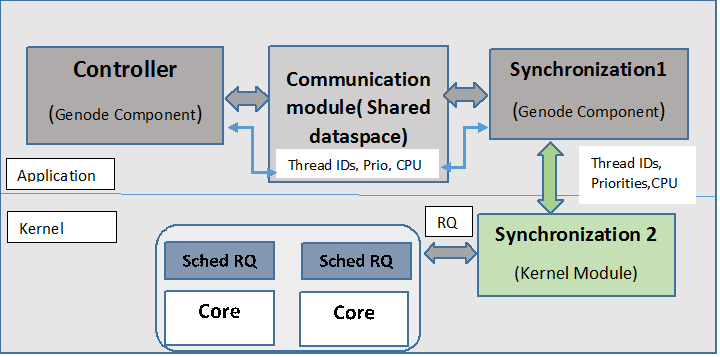
\includegraphics[width=0.7\linewidth]{figures/Abstract_design.png}
	\caption{The synchronization modules design with communication module and Controller}
	\label{fig:abstractdesign}
\end{figure}


The high-level view of the new design is depicted in figure \ref{fig:abstractdesign}.
The Synchronization module is split into two major parts. The first part is implemented as a high-level Genode component, which is responsible for communicating with the \texttt{Controller} and passing the data to the second part. The \texttt{Controller} and the \texttt{Synchronization} module interaction is that of a producer-consumer relationship. The producer (\texttt{Controller}) produces a thread (or ready queue) and a consumer (\texttt{Synchronization} module) consumes the thread by updating it to the kernel ready queue. This needs a synchronization mechanism to be implemented between these two components (see \ref{rqmodule}).

The second part of the \texttt{Synchronization} module is responsible for taking the thread data from the user-level component and updating the threads to the ready queue. It is implemented in the Genode operating system, with most of the work done in L4/Fiasco.OC microkernel. It has to ensure that the access to the ready queue is synchronized. It should also makes sure that the updated threads execute and the system is in safe state.

Figure \ref{fig:Design_25} shows the data and control flow, and the interfaces between the modules of the new design.

\begin{figure}[h]
\centering
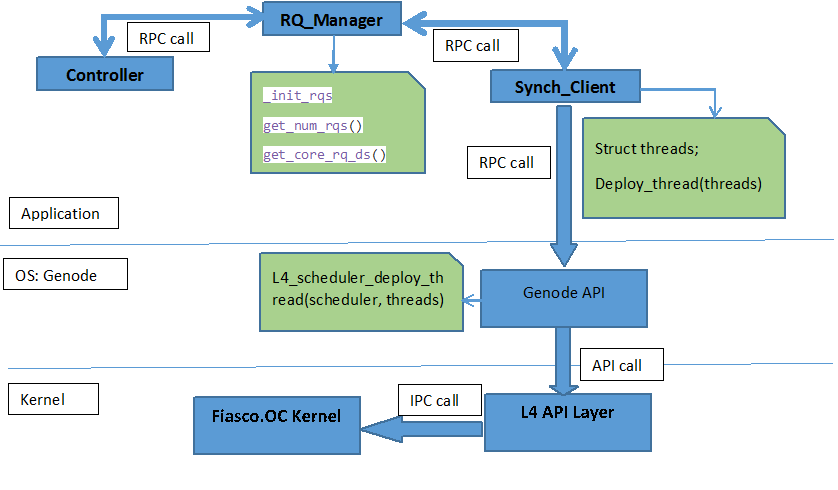
\includegraphics[width=1.0\linewidth]{figures/Design_25.png}
\caption{The data flow between Synch component, Rq manager and Controller}
\label{fig:Design_25}
\end{figure}

The \texttt{Rq\_manager} is a Genode component and is responsible for providing the communication interface between \texttt{Controller} and \texttt{Synchronization}. The main aim is to have a fast communication between the components in order to reduce latency. The best choice for providing a communication interface in Genode is to create a shared dataspace, as explained in section \ref{Foundations:icc}. The \texttt{Rq\_manager} acts as a server in Genode by providing its services to the clients. This is the first component created in the execution sequence, and it provides RPC interface to its clients. This component is only required to provide the initial communication interface and dataspace management. The clients which access the server's services can directly communicate with each other once they obtain the shared dataspace. 

The \texttt{Controller} and the \texttt{Synch\_client} are Genode components and act as clients to the \texttt{Rq\_manager}. The \texttt{Controller} uses the Genode RPC calls to obtain the dataspace capability from \texttt{Rq\_manager}. Once it has the access, it updates the dataspace with thread information. This information consists of the Genode OS framework thread ids, processor id on to which the thread is to be scheduled, and the priorities of the threads. However, the \texttt{Controller} doesn't enforce any policies to the \texttt{Synch\_client}. So, both these components work independently from each other but are synchronized via dataspace.

The \texttt{Synch\_client} also uses the Genode RPC calls to obtain the dataspace capability from \texttt{Rq\_manager}. Once it obtains the access to shared dataspace, it checks for the thread information and transfers the thread ids, priorities and CPU information to the kernel. The communication between Genode and Fiasco.OC kernel is governed by L4 API calls. However, the \texttt{Synch\_client} being a high-level Genode component, cannot make use of L4 API calls by itself. In order to communicate with the kernel, the \texttt{Synch\_client} makes use of Genode OS framework's service. It first creates Genode's RPC object, then using this, it makes a call to the API of Genode's RPC object. The Genode's RPC object makes an API call to the L4 layer. The L4 API communicates the information to Fiasco.OC kernel object by using the IPC service provided by the kernel. The kernel threads are identified by the kernel and updated to the ready queue.

The following sections give detailed design of the individual modules.

\section{Rq\_manager Module}\label{rqmodule}
The communication part of the work was collaborated with Paul Nieleck, who worked on the \texttt{Controller} part of the \texttt{Observer-Controller} architecture\cite{paul}. As Nieleck designed and implemented this module, only the details that help to understand the \texttt{Synchronization} component are described below. 

The \texttt{Rq\_manager} has two main functionalities. First, creating a shared dataspace using Genode's APIs and providing a mechanism to access and modify the shared dataspaces to its clients. The \texttt{Rq\_manager} acts as a server in Genode's client-server relationship. It interacts with the Core's RAM service and obtains a RAM dataspace. The Core’s RAM service returns a dataspace capability after allocating memory. Then, the \texttt{Rq\_manager} attaches the dataspace to its RM session and whenever a client requests this dataspace capability, the server delegates it. Once the clients obtain the dataspace capability, they can attach it to their own RM session and access the contents inside the dataspace. Now, both the server and clients have access to shared memory via their respective virtual addresses.

\section{Synch\_client Module}
The \texttt{Synch\_client} module is a Genode component that is responsible for updating the threads to the ready queue. It communicates with the \texttt{Controller} using a shared dataspace created by the \texttt{Rq\_manager}. This acts as a client to the \texttt{Rq\_manager} and obtains the dataspace capability from the \texttt{Rq\_manager} via an RPC call. It does so by creating a Connection object provided by the \texttt{Rq\_manager}. This is also responsible for transferring the thread update information to the kernel.

Once the dataspace is accessible, the \texttt{Synch\_clinet} runs in an infinite loop to continuously check the dataspace for any thread that needs to be scheduled. Once it finds such a thread, it updates the thread to the ready queue and then, informs the \texttt{Controller} about the scheduling by updating the shared dataspace. This way, the \texttt{Controller} knows whether the thread scheduling was successful.

The \texttt{Synch\_client} also communicates with the kernel. However, this is done by using the Genode's Trace service. It creates a Connection object provided from the Genode's Trace service to make an RPC call to the Trace object. It makes RPC call with the thread information and waits for the call to return. The return value indicates the success/failure about updating the threads to the kernel ready queue. The \texttt{Synch\_client} then updates this information to the shared dataspace so that the \texttt{Controller} can take a scheduling decision.

\section{Ready Queue Update Mechanism} \label{design:rqupdate}

R	eady queue update mechanism is the process of reading the ready to execute threads and making sure that they are updated in the respective ready queues of the processors. Figure \ref{fig:class_rqupdate} shows the high level overview of the involved classes in this process.

\begin{figure}[h]
\centering
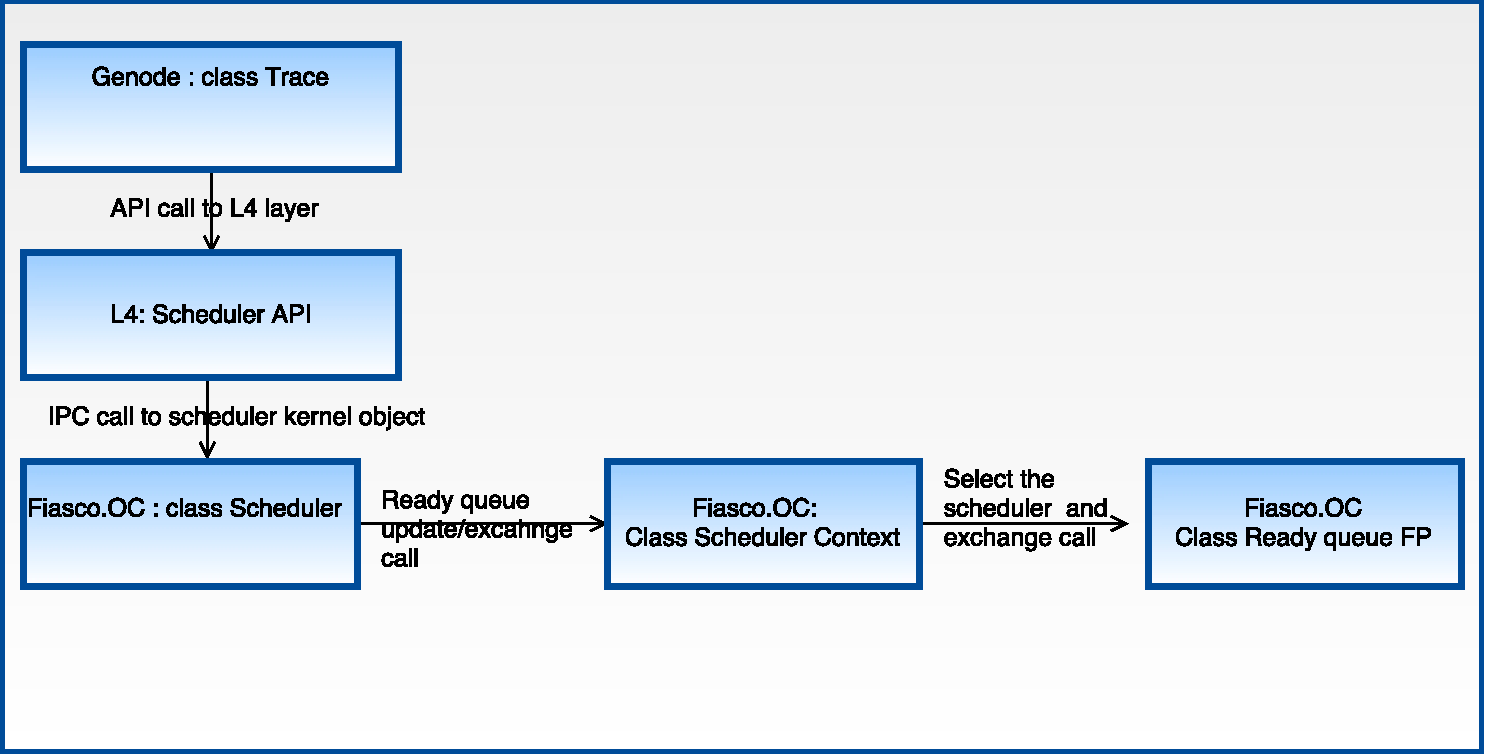
\includegraphics[width=0.9\linewidth]{figures/class_rqupdate1}
\caption{Involved classes in ready queue update meachsnism}
\label{fig:class_rqupdate}
\end{figure}


A Genode module provides an API, which can be called from the \texttt{Synch\_clinet}. The L4 module provides API calls, which can be called from Genode. The Fiasco.OC kernel module accesses the incoming threads and updates them to the ready queue.

The following subsections give an overview of the modules involved in ready queue update mechanism.

\subsection{Genode Module}
Genode module is a component which provides an API that can be called from the \texttt{Synch\_client} to communicate with L4/Fiasco.OC kernel. Since L4 calls cannot be made directly from the application, a Genode helper component is necessary to make these calls. The Genode API acts as a wrapper to the L4 calls. It takes the information from the \texttt{Synch\_client} and copies it to the data structure used by the kernel and calls L4 API. The call to L4 is a blocking one. It waits for the L4 call to return and checks for the success or failure. Based on the return value of the L4 API, the Genode module returns 1 (ready queue update successful) or 0 (ready queue update failure) to the \texttt{Synch\_client}.

\subsection{L4 Module}

The L4 module represents the L4 API layer, which governs the communication between Genode and Fiasco.OC. It provides an API written in L4sys code, which is called from the Genode module. It is responsible for obtaining the thread ids from Genode and pass them to the Fiasco.OC module using an L4 IPC call. The L4 provides many facilities to the kernel, such as utilities for different platforms, GCC libraries and L4 system calls (L4sys). Once the thread ids are obtained from the Genode API, it extracts and fills them in the kernel's UTCB(used for transferring function call parameters) to make the IPC call.

Additionally, the L4 module is also responsible for converting the thread ids to kernel understandable flex pages (explained in \ref{imp:l4api}). Once the IPC call returns, this module returns the same value to the Genode module. 

\subsection{Fiasco.OC Kernel Module}

The Fiasco.OC kernel module is responsible for receiving the threads from the L4 API and safely updating them to the ready queue list of the scheduler. There were two design choices available to receive the incoming threads from L4 API. The first one was to use an existing kernel object (scheduler) and the second was to create a new kernel object (see \ref{implement:kernelobject}). The second method ensures that the legacy code is clean and provides a dedicated object. However, it uses extra memory and adds the complexity of maintaining one more kernel object. So, the idea of using the scheduler object was used in designing this module. The figure \ref{fig:kernel_class} shows the involved classes, data and control flow between these classes in the kernel module.

\begin{figure}[h]
\centering
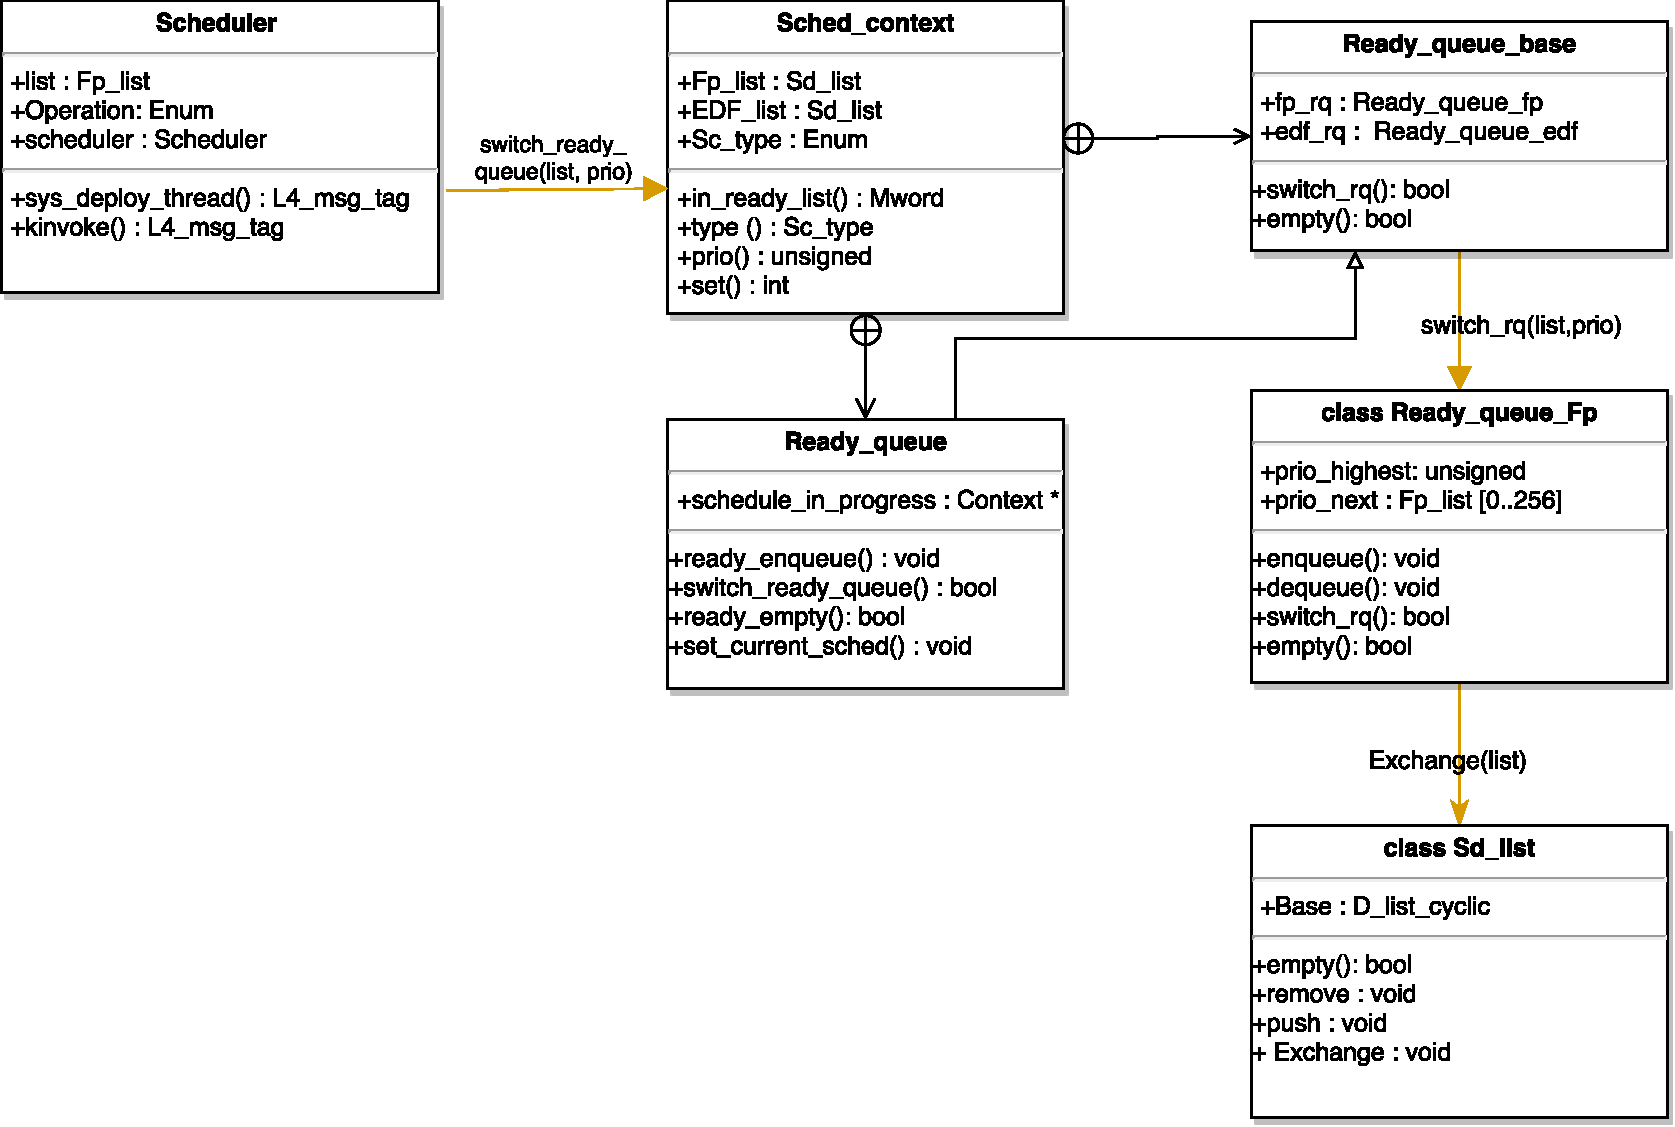
\includegraphics[width=1.0\linewidth]{figures/kernel_class}
\caption{Class diagram of the involved classes (yello arrows show the function calls)}
\label{fig:kernel_class}
\end{figure}

The Scheduler class is in \textit{foc/kernel/fiasco/kern/src} and has a static variable \texttt{scheduler}, which represents the kernel object. The Scheduler context and Ready queue classes implementation is quite complicated. The class \texttt{Sched\_context} is the central class. The \texttt{Ready\_queue} and the \texttt{Ready\_queue\_base} classes are nested inside the \texttt{Sched\_context} class. Also the \texttt{Ready\_queue\_base} class is inherited by \texttt{Ready\_queue} and has both FP and EDF ready queue objects.

%The \texttt{switch\_ready\_queue} function in \texttt{Ready\_queue} makes a call to \texttt{switch\_rq} method, which is inside the \texttt{Ready\_queue\_base}. Here the type of the scheduler is checked and a corresponding ready queue is selected to forward the call. The switch\_rq method inside the Ready\_queue\_fp class exchanges the list using the function from \texttt{sd\_list} class implementation.

The scheduler kernel object is used to get the thread data from the L4 API. The obtained thread information is in the form of L4 flex pages. These pages are converted to get the thread ids, which can be used to obtain the scheduler context objects. A list is created similar to the ready queue list using the scheduler context objects. This module then makes a decision about when the ready queue should be updated according to the current state of the system. After the decision, it makes \texttt{switch\_ready\_queue} function call of the \texttt{Sched\_context} class to switch or update the ready queue.

The call is then transferred to the \texttt{Ready\_queue} class. The type of the ready queue is selected depending on the type of the scheduler in use. If it is a Fixed priority scheduler, the \texttt{switch\_rq} call is made to the \texttt{Ready\_queue\_fp} class. The \texttt{switch\_rq} call receives the new ready queue list and the priority. A call is made to the \texttt{sd\_list} class to switch the ready queue. A boolean value is returned to the scheduler to indicate the success.

Additionally, this module has to provide a synchronized access to the ready queue. The synchronization method used is explained in \ref{imp:sync}. 

\subsection{Finding the Right Time for Ready Queue Update}\label{design:time}
Finding the right point for synchronization is a big challenge. Since this toolchain is used on a safety critical system, care should be taken to ensure that the system remains in a safe and predictable state. Theoretically, the points for safe update of the ready queue are:

\begin{itemize}
\item Empty ready-queue: If the run queue is empty, exchanging the list is easy since no threads exist in the ready queue. In case there is a single thread in the queue, the thread must be an idle thread. So, in the idle thread and empty queue cases,it is safe to exchange the entire ready queue list with a new list. A CPU lock is used to disable the thread preemption and the ready queue list is exchanged.

\item Static point-in-time: In this method, the \texttt{Controller} decides which thread should be allowed to complete its execution before exchanging the ready queue list. The controller can either wait or preempt the currently executing thread.

\item Variable point-in-time: In this method, the synchronization mechanism is used is such way that it takes a decision to pick the best to update the ready queue. If RCU is used, then the update happens after the grace period. If STM is used the transaction is committed if there is no thread is accessing the ready queue (see \ref{rq:sync}).

\end{itemize}
